\documentclass[12pt, a4paper]{article}
\usepackage[utf8]{inputenc}
\usepackage[T1]{fontenc}
\usepackage{lmodern}
\usepackage[dvipsnames]{xcolor}
\usepackage{fancyhdr}
\usepackage{reledmac}
\usepackage{float}
\usepackage{graphicx}
\usepackage{wallpaper}
\usepackage[top=2.5cm, bottom=2cm, left=2cm, right=2cm, heightrounded, marginparwidth=3.5cm, marginparsep=0.3cm]{geometry}
\renewcommand{\headrulewidth}{0.1pt}
\renewcommand{\footrulewidth}{0.3pt}
\usepackage{hyperref}
\pagestyle{fancy}
\lhead{{\scshape{Mével}} Adrien M2 EdNitl}
\chead{}
\rhead{2022-2023}
\fancyfoot[]{}
\rfoot{\thepage}
\usepackage[french]{babel}
\setlength{\headheight}{20.61049pt}

\begin{document}
\ULCornerWallPaper{0.23}{img/logo_u_lille.png}


\begin{titlepage}
  

\vspace*{3cm}

 
\begin{center}
\textsc{\huge Mémoire de recherche}

\textsc{\textit{Pour un nouveau roman}, axes de lectures, projet d'édition numérique}



%Version du 
\today


\vspace*{2cm}
Mme~Florence~\textsc{de Challonge}


M.~Matthieu~\textsc{Marchal}




\vspace*{11cm}
\small
\textsc{Mével}~Adrien

Master~2 Lettres Modernes,

«~Éditions numériques et imprimées de textes littéraires~»

\vspace*{2.5cm}
Année universitaire 2022-2023




\end{center}


\end{titlepage}	

\begin{center}
\end{center}
\vspace{3cm}
\newcommand{\punr}{\textit{Pour un nouveau roman}}
\newcommand{\robbe}{Alain~Robbe-Grillet}

\section{Méthode de réflexion}

Quels éléments doit apporter une édition critique de \punr{} pour permettre la meilleure lecture possible à son lecteur~? 

En soit, le texte ne paraît pas poser de difficulté particulière~: sa langue n'est pas éloigné de la nôtre, la pensée en est claire. Dès lors la question n'est peut-être pas tant de rendre accessible mais de permettre de faire lire plus que le texte~: les possibilités de l'œuvre au sens où, lue comme un manifeste l'œuvre \punr{} est un seuil vers des possibles.

Encore connu du public et facile d'accès, le texte peut être un point d'entrée dans une époque de la littérature où un auteur s'empare des colonnes d'un quotidien généraliste pour y défendre sa théorie littéraire semaine après semaine annonçant une littérature encore à venir aussi bien qu'une initiation à la théorie littéraire.

Donner à lire une époque, établir un texte dans ses environnements multiples permettre une lecture complète au néophyte et produire un outil efficace pour les chercheurs, tels sont les défis que tentent de relever l'édition que nous proposons.


%mentionner le fait qu'on a la chance d'avoir lu les textes cités, besoin de tirer partie de cela

%identifier les articles, la découverte de la thèse de Mme Yanochevski nous fut ici d'une grande aide.

%




\section{Problématique : un texte composite}

Constitué par un regroupement de textes publiés aux fils des années selon des modalités différentes (tantôt dans des revues spécialisées tantôt dans des journaux généraliste) pour des projets (polémiques ou théoriques) particuliers, \punr{} est une œuvre composite. Des critiques d'ouvrages pas toujours contemporains, des textes de théorie littéraire voire même de métaphysique ou de phénoménologie~; cet ouvrage dont on ne perçoit pas toujours l'unité est pourtant loin d'un recueil dans lequel chaque article pourrait se lire indépendamment des autres, réunis par commodité plus que nécessité en un livre unique permettant au grand public de s'approprier les nouveautés de la recherche. En effet quelques fils directeurs traversent et animent les textes~: des références spécifiques témoignage d'une époque littéraire, un style polémique, une pensée somme toute entière et constituée~; l'œuvre tient par un effort, au demeurant moindre et \textit{a posteriori}, d'unification via l'insertion de seuil et les réécritures partielles.

Des récriminations contre «~les critiques~» à un air du temps phénoménologique critique de la métaphysique classique en passant par une certaine vision du bon-sens, l'œuvre qui se présente comme n'étant pas une théorie du roman semble pourtant (re)tracer une voie à la littérature de son époque. \punr, qu'est-ce~? Les propos épars d'un relativement jeune auteur tentant d'occuper le terrain et de promouvoir ses textes~? Un moment de Robbe-Grillet~? Une époque de l'histoire littéraire~? Un livret de recommandations (aux publics, aux critiques, aux auteurs)~? Ou bel et bien une doctrine littéraire~?

Si le texte peut être lu comme tout cela à la fois, cela tient sans doute à la complexité d'une pensée faite de recoins. Tentant de maintenir un équilibre délicat entre légitimation par la tradition et refus d'une autre tradition, entre l'affirmation de ce qu'il ne faudrait pas écrire et le refus de délivrer les consignes de la nouvelle école, \punr{} réfute et emprunte (explicitement ou non) aux modèles et aux adversaires qu'il s'est choisi. L'habileté tenant à un art consommé de l'ironie et du sous-entendu permettant d'emprunter à ceux-là même que l'on entend discréditer.

Déclarant la pleine liberté de l'auteur tout en assénant qu'il ne faudrait plus écrire comme ceci ou comme cela, quelle unité à \punr~? Nous pensons que la pleine compréhension de la manière dont diverses lectures s'imbriquent en un recueil tient à la tenue des fils polémiques et théoriques qui sous-tendent l'ensemble.



    \subsection{Identification et commentaire des articles mis ensemble~: possible critique génétique}
    %\punr est une collection de plusieurs articles publiés dans des journaux et des revues aux profils divers, les réécritures semblent relativement mineures. 
    L'identification et le commentaire des articles originaux ainsi que d'articles connexes qui n'ont pas été retenus dans l'ensemble s'appuieront sur le travail de Mme~Galia~\textsc{Yanoshevsky}\footnote{\textsc{Yanoshevsky} Galia, \textit{Les discours du Nouveau Roman : Essais, entretiens, débats}, Villeneuve d'Ascq, Presses universitaires du Septentrion, 2006} selon laquelle les réécritures semblent relativement mineures. 
    
    %tout en essayant de dégager quelques nouvelles pistes tel le rapport changeant à l'intertexte sartrien.

   %Ce travail sert à l'élaboration d'une base de données qui contiendra entre autre les associations entre les articles originaux et les articles du recueil (voir \ref{db})
%    \subsection{Les raisons de l'ensemble}
%    Recherche d'unité et commentaire des réécritures.
    
    %la constitution de l'ensemble~: thèmes récurrents, résolutions (ou non) d'ambiguïtés au fil des textes.
\newpage


\section{Axes de lectures~: les raisons de l'ensemble}


\subsection{Un style polémique}
%thèse antithèse. Un art de la réfutation
Analyse stylistique sous l'angle de la rhétorique, notamment autour de la propension quasi systématique à écrire sous la forme~: thèse (des critiques, de l'opinion), antithèse (soit les thèses d'\robbe{} présentées comme le bon sens). 
    \subsubsection{Des adversaires désignés~?}
    %usage de la périphrase
    %glossaire adversaire
    De par sa portée polémique \punr{} se désigne des adversaires. Parmi lesquels on trouve~: les critiques généralement non nommés (à quelques exceptions près) et désignés par une expression «~les critiques~» ils sont l'adversaire privilégié et assimilés aux porteurs d'une \textit{doxa} à laquelle le texte s'oppose. Leurs propos réels ou supposés sont mis en valeur tout au long du texte et constituent l'un des points saillants que notre édition entend mettre en évidence (voir \ref{gloss}).
    
    D'un point de vue stylistique outre l'usage du discours indirect libre, de la citation (réelle ou fictive) on distingue l'usage de la périphrase pour désigner sans nommer, englober sans nuance les thèses adverses.

    Par ailleurs les adversaires nommés ou désignés de manière si précises que l'implicite s'expose en procédé rhétorique, semblent constituer des exempla de groupes adversaires. Ainsi Sartre dont l'éloge nuancé pour \textit{La Nausée} semble exemplum du groupe «~socialistes révolutionnnaires~».

    Enfin notre étude entend dégager les raisons théoriques qui organiser la distribution des bons et des mauvais points par \robbe{} aux œuvres citées (telles \textit{La Nausée}, \textit{L'Étranger}, \textit{Le Parti pris des choses})  et aux critiques.
    \subsubsection{Une certaine vision du bon sens}
    %défaire l'habitude.
    De par sa structure, ses arguments à la fois rhétoriques mais également théoriques (où ce que l'on serait tenté d'appeler «~la bonne foie~» est l'un des concepts opérant la distinction), \robbe{} se place comme le tenant du bon sens.

    Or, ce concept de «~bon sens~» mérite d'être interrogé, du moins défini. Si tous s'en réclament, chacun y projette un rapport particulier au savoir. Dans le cas d'\robbe{} le bon sens n'est pas la \textit{doxa}, un avis partagé immédiatement par le plus grand nombre mais bien le résultat d'un dénuement, d'un dévoilement, permettant d'accéder à la vérité (non identique au réel) qui n'étant pas immédiatementdonnée doit faire l'objet d'un travail (de la pensée ou de la forme) pour défaire l'habitude qui prend tantôt l'apparence de clichés tantôt celle de la tradition.

    Nous proposons ici un examen des moyens rhétoriques mais surtout du rapport complexe qu'entretiennent la «~vérité~», du moins la signification, et le réel articulés et explicités dans l'œuvre par le recourt au «~bon sens~». Les moyens de la justification de la position théorique (l'appel au bon sens en tant que dévoilement) coïncide avec la théorie littéraire d'\robbe{} où le réel est ce qui résiste et la signification toujours artificielle.
\subsection{Inscrit dans une époque}
    \subsubsection{Des postulats philosophiques}
    %idée un peu ancienne en vrai
    Si \robbe{} prétend souvent se défaire de la tradition il ne se revendique pas moins d'une certaine tradition. Plus encore cette tradition n'est pas si éloignée de celle qu'il prétend combattre. S'il en appelle à Kafka, Flaubert et Proust comme précurseurs de la modernité contre un certain réalisme et une vision (une écriture) romantique (le terme n'est jamais employé et sa convocation ici fera l'objet d'une justification). Il n'en demeure pas moins qu'une vision de l'auteur comme démiurge et de l'art comme porteur de signification sont des postulats hérités du XIX\textsuperscript{e} siècle.

    Par ailleurs la dialectique sous-tendant la réfutation puis la réapropriation du terme «~formalisme~» s'articule sur le rejet d'une première définition de ce terme (plus ou moins équivalente à la formule de «~l'art pour l'art~») qui rapproche \robbe{} de ses détracteurs (réels ou fictifs) et la reconstitution d'une définition plus proche de la forme sens.
    \subsubsection{Et de vagues références contemporaines}
    %s'inscrit dans une époque
    %barthes
    %la critique de la pensée positiviste et occidentalisme
    %libertaire
    Inscrit dans son époque, \punr{} mobilise des références contemporaines à son époque qui nourrissent et appuient la démonstration. Certaines relativement explicites~: Barthes, Heidegger~; d'autres plus diffuses et plus symptomatique de l'époque~: la critique du positivisme, une vision libertaire des droits de l'auteur, la récente tradition phénoménologique.

    Enfin l'intertexte Sartrien, en premier lieu \textit{Qu'est-ce que la littérature} adversaire désigné et combattu à certains passages presque mot à mot semble une source d'inspiration tout aussi fondamentale pour l'élaboration des thèses (voire même le style) défendues par \robbe~: si \punr{} réfute la formule «~on n'écrit pas pour rien dire~» il n'en demeure pas moins qu'\robbe{} défend une vision du travail de la forme créateur de sens, ce qui n'est pas très différent des idées de Sartre.
\subsection{Une véritable théorie esthétique~: l'écart(~?)}
    \subsubsection{L'innovation contre l'habitude}
    
    Le recueil \punr{} n'est pas tant une théorie dont on peut tirer des recommandations qu'une théorie de ce qu'il ne faudrait pas écrire.
    
    Le Nouveau Roman présenté comme une recherche cherchant à étendre les possibilités d'écriture n'a pas de point d'arrivée mais un point de départ~: les romans supposés balzaciens. Dès lors \punr{} mesure la valeur des quelques exemples ou préceptes qu'il nous donne en fonction de leur distance vis-à-vis de la tradition. Ceci étant dit il reste à bien mesurer à quel point cet écart est perçu comme une évolution diachronique en laquelle on distingue une idée de progrès ou bien un écart entre une littérature peu exigeante perçue comme réactionnaire.

    
    \subsubsection{Un anti-roman ?}
    Alors même que Robbe-Grillet refuse cette appelation «~d'anti-roman~», les innovations qu'il vante le sont toujours en tant qu'innovation contre un modèle, supposé.

    La poétique d'\robbe{} est une théorie du renouvellement plutôt que de l'approfondissement~: si \punr{} cherche des précurseurs au Nouveau Roman, il les présente comme des ruptures dont l'actualité est maintenue par un art littéraire rétrograde.

    %Thomas Pavel Pensée du roman. 2003 !
     \subsection{Quel héritage à \punr{}~?}
        \subsubsection{Les emprunts, liens avec les écrits théoriques des autres membres du Nouveau~Roman}
     %\subsubsection{Les emprunts à Butor/Sarraute ou autre}
    Avant d'être un héritage possible \punr{} est un héritier des écrits théoriques de Sarraute notamment. Une part importante du travail consiste en l'identification et le commentaire d'emprunts et de signes manifestes d'influence d'autres textes publiés par le groupe au sein du recueil.     
     
         \subsubsection{\punr{} et les nouveaux-romanciers référence ou repoussoir~?}
    Quels rapports entretinrent les autres membres du groupe au recueil~? Y firent-ils explicitement référence ou non~?

    Nous nous pencherons sur les propos et ouvrages des autres membre du mouvement à la recherche de liens permettant d'identifier la réception de \punr{} par les autres néo-romanciers. Cette analyse permettant également de questionner l'électivité du «~manifeste~».

%    De cela nous avons au moins un exemple~: Ricardou dans 

         \subsubsection{Une théorie qui fit date ?}
     Élargissement de la question de la posterité du texte~: a-t-il eu des héritiers déclarés~? Les thèses d'\robbe{} ont-elles été reprises en dehors du cercle des auteurs du mouvement~?
     
     
     

\newpage

\section{Éléments d'une édition numérique}
Pour donner à lire le texte~: production d'une édition HTML par un encodage XML-TEI via DTD ou ODD, l'odd offrant l'avantage de permettre une documentation des choix d'encodages et une insertion plus forte dans le standard de la TEI mais est nettement plus longue à réaliser. Les modalités précises (encodage des variantes, des référents intertertextuels et de l'apparat critique restent à définir).


L'édition numérique se proposerait de diviser les articles de \punr{} et d'en proposer une lecture "éclatée" tel découpage mérite commentaire~: 
\begin{enumerate}
    \item Après une présentation générale, une présentation accompagnera chaque article au sein de ces présentations~: grand renfort de liens hypertextes créant des passerelles entre la présentation et des paragraphes/sections numériques annexes et connexes.
    \item Adaptation légère de la table des matières et de l'organisation du texte insistant davantage sur l'aspect hétéroclite du texte. Plutôt qu'une lecture continue, nous nous efforcerions de produire un texte dans lequel on peut piocher et lire telle ou telle partie en fonction des besoins.
    \begin{enumerate}
        \item Le texte d'introduction aux «~Éléments d'une anthologie moderne~» accompagnera chacune des sous-sections constituant l'ensemble plutôt qu'un texte indépendant. (Il sera sans doute conçu sur le modèle <summary/detail> en HTML pour permettre de le faire apparaître/disparaître en un clic).
        \begin{itemize}
             \item Dans la table des matières de l'édition papier les différents «~Éléments d'une anthologie moderne~» seront traités comme des sous-parties de niveau équivalent aux «~notions périmées~» (Le personnage, l'histoire etc.) ce n'est pas le cas dans le corps de l'ouvrage. Les titres courant en haut de page correspondent aux «~éléments~» mais pas pour les notions.
            \item Les «~éléments~» se signalent au regard du lecteur comme des textes indépendants de critique littéraire (objet d'une première publication retravaillée pour certains) et ont bien la longueur d'articles indépendants.
            \item Les «~notions~» sont bien plus courtes et sont présentées comme des sous-parties.
        \end{itemize}
        \item Chacun des articles offrira une table des matières (sur la droite ou sur la gauche) qui permet de passer d'une section à une autre. Par exemple~: chacune des «~notions~» faisant l'objet d'une sous-partie dans le texte original et non d'un article sera conservé telle quelles, un petit menu permettant d'aller en un clic de «~personnage~» à «~histoire~».
        \begin{itemize}
            \item Jusqu'où ira-t-on~? On peut aussi aller jusqu'à découper chacun des articles en fonction de partie ou de mouvements repérés au cours de la recherche. Par exemple~: un des traits caractéristiques de l'écriture de Robbe-Grillet tout au long du recueil est de vider l'argumentation très tôt (généralement les premières lignes de l'article) résumant les thèses adverses comme s'il s'agissait de la \textit{doxa} avant de s'opposer aux adversaires qu'il s'est ainsi créés. Est-il pertinent d'offrir une démonstration via table des matières de ce point en créant des sauts vers "exposition de la thèses adverse", "réfutation"~? 
        \end{itemize}
        
    \end{enumerate}
    \label{gloss}
    \item Un "glossaire des adversaires". Tout au long du texte un point qui nous paraît mériter d'être illustré est l'emploi des guillemets. Outre l'emploi classique pour marquer des citations, Robbe-Grillet fait un usage polémique des guillemets référençant ce que l'on pourrait appeler les termes usuels de la critique. 
    \begin{itemize}
        \item Un tel glossaire serait justifié dans le travail de recherche.
        \item Les termes sont repérables à l'emploi de guillemets qui servent aussi à marquer les citations, si ces termes sont également des citations, leur statut diffère en ce qu'elle sont des citations créées par Robbe-grillet, des propos supposés. Dès lors il conviendra de justifier les passages entre guillemets exclus de ce "glossaire".
       % \item C'est un fait \textbf{quasi}-systématique tout au long de l'ouvrage. Dès lors justifications nécessaires pour les moments du textes où cette sorte de glossaire n'est plus alimenté/able.
    \end{itemize}
    \item Un "glossaire des expressions préférées". Autre trait saillant qui répond directement au précédent~: Robbe-Grillet inscrit en italique quelques formulations qu'il entend promouvoir. Généralement issues d'un plus ou moins long mouvement de réfutation, une correspondance terme à terme avec le "glossaire des adversaires" ne paraît pas tout à fait envisageable mais la possibilité doit être étudiée. Nous entendons par là mettre l'accent sur deux choses~:
        \begin{itemize}
            \item Robbe-Grillet ne se présente pas comme un idéologue mais comme un penseur et se revendique du bon sens. Cette manière de montrer la pensée en train de se faire et se fixant après examen sur des "formules clefs" nous paraît un trait caractéristique qui a l'avantage de pouvoir proposer une expérience de lecture ludique et synthétique, scientifiquement valide et pratique.
            \item La nature dichotomique de l'ouvrage et de l'écriture. L'essai dans son ensemble est extrêmement polémique dans son style même, exposition/réfutation, thèse/antithèse s'enchaînent et le lecteur ne perçoit que difficilement des efforts de synthèse. La paroxysme semblant «~Nouveau roman, homme nouveau~» construit le plus clairement possible sur des assertions catégoriques présentées par couple dichotomique.
        \end{itemize}
    \item Mises en valeurs des relations intertextuelles.
    Dans l'idéal nous souhaiterions produire une édition qui serait en mesure de permettre une découverte ou une vérification des références citées.

    Cette mise en valeur aurait l'intérêt de permettre à un lectorat non spécialiste d'avoir accès à plutôt que la seule citation produite par \robbe{} et son commentaire à un segment plus important de l'œuvre citée~: le contexte de l'élément dont \robbe{} tire argument et à un lectorat plus expert de vérifier et juger l'usage qu'en fait \robbe{}, et plus généralement, approfondir la réflexion.
        \begin{itemize}
            \item Avantages~:
            \begin{itemize}
                \item Une telle solution pourrait être très plaisante~: le passage référent (citation plus ou moins explicite) serait mis en valeur par un jeu de couleur et par le clic de l'utilisateur un extrait se superposerait au texte de \punr{} et serait lui-même congédiable en un clic.
                \item Cette démarche transformerait l'édition en une véritable machine à lire et ouvre le tissu textuel sur son environnement.
            \end{itemize}
            %lu la plupart des textes cités
            
            \item Inconvénients~:
            \begin{itemize}
                \item L'identification des passages peut être difficile et surtout prendre du temps. En effet identifier tel ou tel passage de \textit{La Conscience de Zeno} cité (de manière approximative~?) sans mention de page par \robbe{} dans une traduction sans doute différente demande un investissement conséquent en temps.
                \item Quelques cas limites posent également problème. \robbe{} cite souvent «~Proust~» et «~Flaubert~» sans spécifier un passage particulier. Faudrait-il alors se garder de proposer un passage pour privilégier une présentation de l'auteur~; laquelle risquerait d'être davantage une collection de lieux communs à l'intérêt limité ou privilégier un commentaire argumenté sur la lecture que propose \robbe{} de ces auteurs~? Par ailleurs, certaines références telles Sarraute, Sartre ou Butor ne sont pas explicitement citées mais relèvent plutôt d'emprunts implicites qui compliquent encore l'identification et introduisent des degrés divers de références pour lesquels il conviendrait d'opérer un traitement différent/
                \item Enfin, outre les difficultés techniques ce travail induit une relative lourdeur du déploiement au vu de la quantité d'intertextes identifiables qui risque plutôt que de faciliter la lecture de détourner le lecteur de l'œuvre première.
            \end{itemize}
            %identification des passages
            %limites des cas où l'intertexte est "Flaubert" ou "Pourst" Dans ces cas présentation de l'auteur~? Et si présentation de l'auteur, on se retrouve vite à énoncer des banalités sur Proust ou Flaubert --> dès lors privilégier qqh comme "les lectures que les nouveaux romanciers font de ces auteurs" avec passages cités de Sarraute par ex. sur flaubert et proust ou butor ?
            %difficulté techniques et lourdeurs effectives du déploiement
            %délimitation des relations. Outres les cas où la citation est lâhée sans trop de contexte pensont au cas où il cite Butor (check) et au cas où Simon parle aussi de roman filmique dans interview sur youtube, et tout l'intertexte sartiren fondamental qui n'est pas toujours "explicitement" cité.
        \end{itemize}
        \item Une base de données offrant une visualisation des relations intertextuelles au sein des articles \label{db}. Cette base de données ferait l'objet d'une visualisation synthétique agréable et permettrait en un coup d'œil de relier les intertextes aux articles auxquels ils sont liés tout en indiquant leur statut axiologique et leur degré d'explicitation. Ce travail s'inscrit dans le cours de bases de données animé par Mme~Delphine \textsc{Tribout} et une première version de la base de données a été réalisée mi-décembre et quelques améliorations ou ajustements sont prévus.
\end{enumerate}





   


\subsection{Représentation de l'édition numérique envisagée}



\begin{figure}[H]
    \centering
    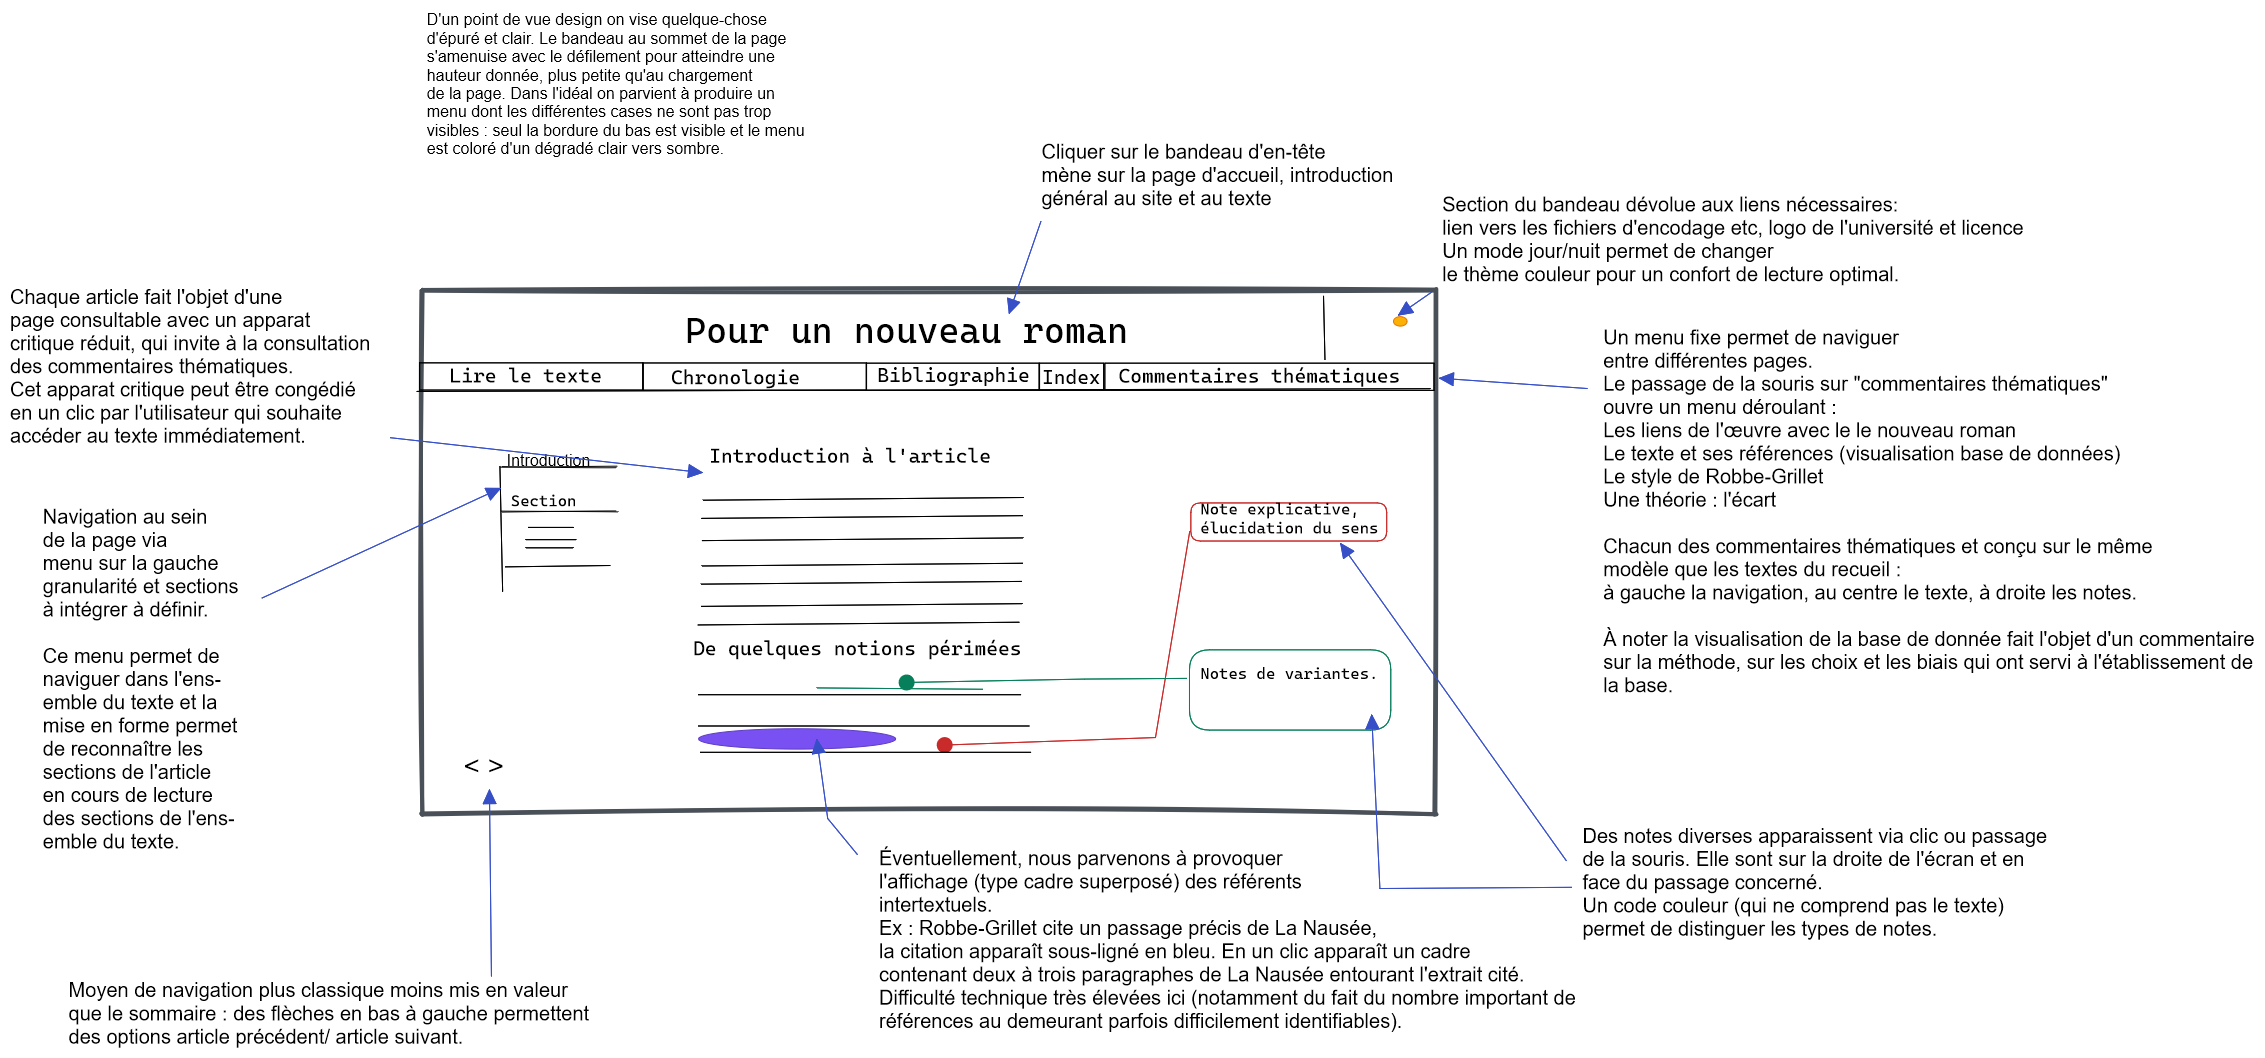
\includegraphics[scale=0.38]{img/202211_mevel_punr_edition_numerique.png}
    \caption{Design et fonctionnalitées d'une édition numérique de \punr{}}
    \label{schema}
\end{figure}

\section{Bibliographie}

\vspace*{2cm}
		\setlength{\parindent}{0cm}
{\large\textsc{Édition citée de Pour un nouveau roman}}
		\vspace*{1cm}
		\setlength{\parindent}{25pt}
		
		
		
		
		\textsc{Robbe-Grillet} Alain, \textit{Pour un nouveau roman}, Paris, Les Éditions de Minuit, coll. «~Double~», 2013 [1963]\par 
		 
		
	
		\vspace*{2cm}
		\setlength{\parindent}{0cm}
{\large\textsc{Œuvres d'Alain Robbe-Grillet citées}}
		\vspace*{1cm}
		\setlength{\parindent}{25pt}
		
		
		
		
		\textsc{Resnais} Alain, \textit{L'Année dernière à Marienbad}, , Silverfilms, Argos Films, Cinétel, Les Films Tamara, Precitel, Société Nouvelle des films Cormoran, Cineriz, Como Films, Terra Film Produktion, 1961\par 
		 
		
	
		\textsc{Robbe-Grillet} Alain, \textit{L'Immortelle}, , Cocinor, Como Films, Dino De Laurentiis Cinematografica, Les Films Tamara, 1963\par 
		 
		
	
		\textsc{Robbe-Grillet} Alain, \textit{Les Gommes}, Paris, Les Éditions de Minuit, 1998 [1953]\par 
		 
		
	
		\textsc{Robbe-Grillet} Alain, \textit{Le Voyeur}, Paris, Les Éditions de Minuit,  [1955]\par 
		 
		
	
		\textsc{Robbe-Grillet} Alain, \textit{La Jalousie}, Paris, Les Éditions de Minuit, coll. «~Double~», 1957 [2017]\par 
		 
		
	
		\textsc{Robbe-Grillet} Alain, \textit{Dans le labyrinthe}, Paris, Les Éditions de Minuit,  [1959]\par 
		 
		
	
		\vspace*{2cm}
		\setlength{\parindent}{0cm}
{\large\textsc{Œuvres d'Alain Robbe-Grillet non citées lues}}
		\vspace*{1cm}
		\setlength{\parindent}{25pt}
		
		
		
		
		\textsc{Robbe-Grillet} Alain, \textit{Djinn}, Paris, Les Éditions de Minuit, coll. «~Double~», 1981 [2018]\par 
		 
		
	
		\textsc{Robbe-Grillet} Alain, \textit{Un Régicide}, Paris, Les Éditions de Minuit, 2006 [1978]\par 
		 
		
	
		\vspace*{2cm}
		\setlength{\parindent}{0cm}
{\large\textsc{Sur le Nouveau Roman}}
		\vspace*{1cm}
		\setlength{\parindent}{25pt}
		
		
		
		
		\textsc{de Chalonge} Florence, \textit{Les Défis du Nouveau roman}, Paris, Canopé, 11/07/2017, p.~64-67\par
		
		
		
		
	
		\textsc{Duval} Romain, \textit{Le formalisme contre les formes}, Paris, Nouvelle revue d’esthétique, 2012/2, p.~141-151
			
			En ligne~: \hyperlink{https://www.cairn.info/revue-nouvelle-revue-d-esthetique-2012-2-page-141.htm}{https://www.cairn.info/revue-nouvelle-revue-d-esthetique-2012-2-page-141.htm}, consulté le \today
		\par
		
		
		
		
	
		\textsc{Milat} Christian, \textit{Sartre et Robbe-Grillet, ou les chemins de l'écriture}, Paris, Revue d'Histoire littéraire de la France, Janvier-Février, 2002, p.~83-96
			
			En ligne~: \hyperlink{https://www.jstor.org/stable/40534639}{https://www.jstor.org/stable/40534639}, consulté le \today
		\par
		
		
		
		
	
		\textsc{Yanoshevsky} Galia, \textit{Les discours du Nouveau Roman : Essais, entretiens, débats}, Villeneuve d'Ascq, Presses universitaires du Septentrion, 2006
			
			En ligne~: \hyperlink{https://doi-org.ressources-electroniques.univ-lille.fr/10.4000/books.septentrion.54734}{https://doi-org.ressources-electroniques.univ-lille.fr/10.4000/books.septentrion.54734}, consulté le \today
		\par 
		 
		
	
		\textsc{Ricardou} Jean, \textit{Le Nouveau Roman suivi de Les Raisons de l'ensemble}, Paris, Éditions du Seuil, coll. «~Points~», 1990 [1973]\par 
		 
		
	
		\textsc{Sarraute} Nathalie, \textit{L'Ère du soupçon}, Paris, Gallimard, coll. «~Pléiade~», 1996 [1956]\par 
		 
		
	
		\vspace*{2cm}
		\setlength{\parindent}{0cm}
{\large\textsc{Critiques généralistes}}
		\vspace*{1cm}
		\setlength{\parindent}{25pt}
		
		
		
		
		\textsc{Hugo} Victor, \textit{Ruy Blas}, Paris, Livre de poche, 2009 [1838]\par 
		 
		
	
		\vspace*{2cm}
		\setlength{\parindent}{0cm}
{\large\textsc{Œuvres citées}}
		\vspace*{1cm}
		\setlength{\parindent}{25pt}
		
		
		
		
		\textsc{Balzac} Honoré, \textit{Le Père Goriot}, Paris, Pocket, coll. «~Pocket Classique~», 1989 [1842]\par 
		 
		
	
		\textsc{Flaubert} Gustave, \textit{Madame Bovary}, Paris, Pocket, coll. «~Pocket Classique~», 1998 [1857]\par 
		 
		
	
		\textsc{Beckett} Samuel, \textit{Molloy}, Paris, Les Éditions de Minuit, coll. «~Double~», 1982 [1951]\par 
		 
		
	
		\textsc{Beckett} Samuel, \textit{Fin de partie}, Paris, Les Éditions de Minuit, 2009 [1957]\par 
		 
		
	
		\textsc{Beckett} Samuel, \textit{En attendant Godot}, Paris, Les Éditions de Minuit, 2007 [1952]\par 
		 
		
	
		\textsc{Camus} Albert, \textit{L'Étranger}, Paris, Gallimard, coll. «~Folio~», 2010 [1942]\par 
		 
		
	
		\textsc{Céline} , \textit{Voyage au bout de la nuit}, Paris, Gallimard, coll. «~Folioplus classiques~», 2011 [1952]\par 
		 
		
	
		\textsc{Dostoïevski} Fédor, \textsc{Markowicz} André (trad.), \textit{Les Fères Karamazov}, Paris, Actes Sud, coll. «~Babel~», 2002 pour la traduction française,  [1880]\par 
		 
		
	
		\textsc{Faulkner} William, \textsc{Coindreau} Maurice Edgar (trad.), \textit{Le Bruit et la fureur}, Paris, Gallimard, coll. «~Folio~», 20071972 pour la traduction française,  [1931]\par 
		 
		
	
		\textsc{Kafka} Franz, \textsc{Nesme} Axel (trad.), \textit{Le Château}, Paris, Librairie Générale Française, coll. «~Le Livre de poche~», 20072001 pour la traduction française,  [1926]\par 
		 
		
	
		\textsc{Kafka} Franz, \textsc{Vialatte} Alexandre (trad.), \textit{Le Procès}, Paris, Gallimard, coll. «~Folio classique~», 20091933 pour la traduction française,  [1925]\par 
		 
		
	
		\textsc{Pascal} Blaise, \textit{Pensées}, Paris, Pocket, coll. «~Agora~», 2009 [1670]\par 
		 
		
	
		\textsc{Proust} Marcel, \textit{Du côté de chez Swann}, Paris, Gallimard, coll. «~Folio classique~», 1988 [1913]\par 
		 
		
	
		\textsc{Queneau} Raymond, \textit{Le Chiendent}, Paris, Gallimard, coll. «~Folio~», 2009 [1933]\par 
		 
		
	
		\textsc{Sartre} Jean-Paul, \textit{La Nausée}, Paris, Gallimard, coll. «~Folio~», 2009 [1938]\par 
		 
		
	
		\textsc{Sartre} Jean-Paul, \textit{Qu'est-ce que la littérature ?}, Parus, Gallimard, coll. «~Folio essais~», 2008 [1948]\par 
		 
		
	
		\textsc{Stendhal} , \textit{La Chartreuse de Parme}, Paris, Pocket, coll. «~Pocket Classiques~», 2008 [1839]\par 
		 
		
	
		\textsc{Roussel} Raymond, \textit{Locus solus}, Paris, Flammarion, coll. «~GF~», 2005 [1965]\par 
		 
		
	
		\textsc{Svevo} Italo, \textsc{Michel Fusco} Paul-Henri Mario (trad.), \textit{La Conscience de Zeno}, Paris, Gallimard, coll. «~Folio~», 20101986 pour la traduction française,  [1954]\par 
		 
		
	
		\textsc{Pinget} Robert, \textit{Mahu ou le matériau}, Paris, Les Éditions de Minuit, 1997 [1952]\par 
		 
		
	
		\textsc{Pinget} Robert, \textit{Le Renard et la boussole}, Paris, Les Éditions de Minuit, 2000 [1953]\par 
		 
		
	
		\textsc{Ponge} Francis, \textit{Le Parti pris des choses}, Paris, Gallimard, coll. «~nrf~», 2013 [1942]\par 
		 
		
	
		\vspace*{2cm}
		\setlength{\parindent}{0cm}
{\large\textsc{Modèle d'édition critique}}
		\vspace*{1cm}
		\setlength{\parindent}{25pt}
		
		
		
		
		\textsc{Duras} Marguerite, \textit{Œuvres complètes}, Paris, Gallimard, coll. «~Pléiade~», 2011\par 
		 
		
	
		\textit{Site du fonds Jean Ricardou} en ligne~: \hyperlink{https://jeanricardou.org/}{https://jeanricardou.org/}, consulté le 23 novembre 2022\par
		
		
		
	
		\textsc{Valincourt} , \textit{Lettres à Madame la marquise *** sur le sujet de La Princese de Clèves}, Paris, Flammarion, coll. «~Garnier Flammarion~», 2021 [1678]\par 
		 
		
	
		\vspace*{2cm}
		\setlength{\parindent}{0cm}
{\large\textsc{Première publication des textes constituants l'ensemble}}
		\vspace*{1cm}
		\setlength{\parindent}{25pt}
		
		
		
		
		\textsc{Robbe-Grillet} Alain, \textit{Il écrit comme Stendhal}, Paris, L'Express, , 1955/10/25, p.~8\par
		
		
		
		
	
		\textsc{Robbe-Grillet} Alain, \textit{La littérature aujourd'hui - VI}, Paris, Tel Quel, n°14, 1963 été, p.~39-45\par
		
		
		
		
	
		\textsc{Robbe-Grillet} Alain, \textit{Une voie pour le roman futur}, Paris, Nouvelle Revue Française, n°43, 1956/07, p.~77-84\par
		
		
		
		
	
		\textsc{Robbe-Grillet} Alain, \textit{Pour un réalisme de la présence}, Paris, L'Express, 1956/01/17, p.~11\par
		
		
		
		
	
		\textsc{Robbe-Grillet} Alain, \textit{Réalisme et révolution}, Paris, L'Express, 1955/01/03, p.~15\par
		
		
		
		
	
		\textsc{Robbe-Grillet} Alain, \textit{Littérature engagée, littérature réactionnaire}, Paris, L'Express, 1955/12/20, p.~11\par
		
		
		
		
	
		\textsc{Robbe-Grillet} Alain, \textit{La Forme et le contenu}, Paris, France Observateur, n°392, 1957/11/14, p.~19\par
		
		
		
		
	
		\textsc{Robbe-Grillet} Alain, \textit{Il n'y a pas "d'avant garde"}, Paris, France Observateur, n°388, 1957/10/17, p.~19\par
		
		
		
		
	
		\textsc{Robbe-Grillet} Alain, \textit{Un joli talent de conteur}, Paris, France Observateur, n°390, 1957/10/31, p.~19\par
		
		
		
		
	
		\textsc{Robbe-Grillet} Alain, \textit{Écrire pour son temps}, Paris, France Observateur, n°387, 1957/10/10, p.~17\par
		
		
		
		
	
		\textsc{Robbe-Grillet} Alain, \textit{Le réalisme socialiste est bourgeois}, Paris, L'Express, 1956/02/21, p.~11\par
		
		
		
		
	
		\textsc{Robbe-Grillet} Alain, \textit{La mort du personnage}, Paris, France Observateur, n°389, 1957/10/24, p.~20\par
		
		
		
		
	
		\textsc{Robbe-Grillet} Alain, \textit{Nature, Humanisme, Tragédie}, Paris, Nouvelle Revue Française, n°70, 1958/10, p.~580-603\par
		
		
		
		
	
		\textsc{Robbe-Grillet} Alain, \textit{Énigmes et transparences chez Raymond Roussel}, Paris, Critique, n°199, 1963/12, p.~1027-1033\par
		
		
		
		
	
		\textsc{Robbe-Grillet} Alain, \textit{La conscience malade de Zeno}, Paris, Nouvelle Revue Française, n°19, 1954/07, p.~138-141\par
		
		
		
		
	
		\textsc{Robbe-Grillet} Alain, \textit{Joë Bousquet le rêveur}, Paris, Critique, n°77, 1953/10, p.~819-829\par
		
		
		
		
	
		\textsc{Robbe-Grillet} Alain, \textit{Samuel Beckette ou la présence sur la scène}, Paris, Critique, n°189, 1963/02, p.~108-114\par
		
		
		
		
	
		\textsc{Robbe-Grillet} Alain, \textit{Samuel Beckett, Auteur dramatique}, Paris, Critique, n°69, 1953/02, p.~108-114\par
		
		
		
		
	
		\textsc{Robbe-Grillet} Alain, \textit{Un roman qui s'invente lui-même}, Paris, Critique, n°80, 1954/01, p.~82-88\par
		
		
		
		
	
		\textsc{Robbe-Grillet} Alain, \textit{Nouveau roman, homme nouveau}, Paris, Revue de Paris, n°68, 1961/09, p.~115-121\par
		
		
		
		
	
		\textsc{Robbe-Grillet} Alain, \textit{Comment mesurer l'inventeur des mesures}, Paris, L'Express, n°627, 1963/06/20, p.~44-45\par
		
		
		
		
	
		\textsc{Robbe-Grillet} Alain, \textit{Monsieur Personne répond... Pour un "nouveau roman"}, Paris, Le Figaro Littéraire, 1963/12/05-11, p.~1-26\par
		
			

\end{document}